\documentclass{article}
\usepackage{graphicx}
\usepackage[dvipsnames,table]{xcolor}
\usepackage[utf8]{inputenc}
\usepackage{siunitx}
\usepackage[american,siunitx]{circuitikz}
\usepackage{amsmath}
\usepackage{svg}
\usepackage{booktabs}
\usepackage{float}
\usepackage{xparse, xfp}
\usepackage{multirow}
\usepackage{tikz}
\usepackage{karnaugh-map}
\usepackage{pdfpages}
\usepackage{hyperref}
\hypersetup{
    colorlinks=true,
    linkcolor=blue,
    filecolor=magenta,      
    urlcolor=cyan,
}
\usepackage{caption} 
\captionsetup[table]{skip=10pt}

\usetikzlibrary{calc}
%\usepackage[landscape]{geometry}
\renewcommand{\thesubsection}{\thesection.\alph{subsection}}
\newcommand{\equal}{=}
\newcommand{\greyrule}{\arrayrulecolor{black!30}\midrule\arrayrulecolor{black}}
\makeatletter
\newcommand\currcoor{\the\tikz@lastxsaved,\the\tikz@lastysaved}
\makeatother
\newcolumntype{:}{@{\hskip\tabcolsep\color{black!30}\vrule\hskip\tabcolsep}}

\ExplSyntaxOn
\NewExpandableDocumentCommand \groupify { O{\,\allowbreak} m m }
  { \jakob_groupify:nnn {#1} {#2} {#3} }
\cs_new:Npn \jakob_groupify:nnn #1 #2 #3
  { \__jakob_groupify_loop:nnw { 1 } {#2} #3 \q_recursion_tail {#1} \q_recursion_stop }
\cs_new:Npn \__jakob_groupify_loop:nnw #1 #2 #3
  {
    \quark_if_recursion_tail_stop:n {#3}
    \exp_not:n {#3}
    \int_compare:nNnTF {#1} = {#2}
      { \__jakob_groupify_sep:n }
      { \exp_args:Nf \__jakob_groupify_loop:nnw { \int_eval:n { #1+1 } } }
          {#2}
  }
\cs_new:Npn \__jakob_groupify_sep:n #1 #2 \q_recursion_tail #3
  {
    \tl_if_empty:nF {#2} { \exp_not:n {#3} }
    \__jakob_groupify_loop:nnw { 1 } {#1}
    #2 \q_recursion_tail {#3}
  }
\ExplSyntaxOff

\title{ECE 2200L\\Introduction to Microelectronics Circuits Laboratory\\\,\\Experiment 7\\MOSFET Transistor Current-Voltage Characteristics\\\,\\Report}
\author{Choi Tim Antony Yung}
\date{October 28, 2020}
\begin{document}
\maketitle

\thispagestyle{empty}
\setcounter{page}{0}

\newpage

\section*{Objective}
To study the transfer characteristics of the Metal Oxide Semiconductor Field Effect Transistor (MOSFET) through laboratory experimentation.

\section*{Procedure}
The following is the set up for this experiment.
\begin{figure}[H]
  \centering
  \begin{circuitikz}
    \draw
    (0,0)node[nigfete](Q){}
    (Q.S)node[ground]{}
    (Q.G)--++(-1,0)to[V_=$V_{GS}$]++(0,-2)node[ground]{}
    (Q.D)to[R=\SI{300}{\ohm},i<=$I_D$]++(3,0)to[battery1, v=$V_{DD}\equal\SI{5}{\volt}$]++(0,-2)node[ground]{}
    ;
  \end{circuitikz}
  \caption{Circuit 1 to determine $V_{TH}$}
  \label{fig:ckt1}
\end{figure}

\begin{figure}[H]
  \centering
  \begin{circuitikz}
    \draw
    (0,0)node[nigfete](Q){}
    (Q.S)node[ground]{}
    (Q.G)--++(-1,0)to[V_=$V_{GS}$]++(0,-2)node[ground]{}
    (Q.D)to[R=\SI{300}{\ohm},i<=$I_D$]++(3,0)to[V=$V_{DD}$]++(0,-2)node[ground]{}
    ;
  \end{circuitikz}
  \caption{Circuit 2 to determine IV relationship}
  \label{fig:ckt2}
\end{figure}

\newpage

\section*{Result}
The following data is obtained from circuit 1.

\begin{table}[H]
  \caption{$I_D$ vs $V_{GS}$ of circuit 1 at $V_{DS} = \SI{5}{\volt}$}
  \centering
    \begin{tabular}{rrrr}
      \toprule
       $V_{GS}$ (V)&$I_D$ (A)&$\sqrt{I_D}$ $(\sqrt{A})$\\
      \midrule
      1.500 & $2.92\times10^{-5}$ & 0.005404 \\
      1.812 & $1.69\times10^{-3}$ & 0.041110 \\
      2.003 & $1.12\times10^{-2}$ & 0.105877 \\
      2.090 & $2.16\times10^{-2}$ & 0.146969 \\
      2.137 & $2.92\times10^{-2}$ & 0.170997 \\
    \bottomrule
  \end{tabular}
  \label{tab:ckt1}%
\end{table}

\begin{figure}[H]
  \centering
  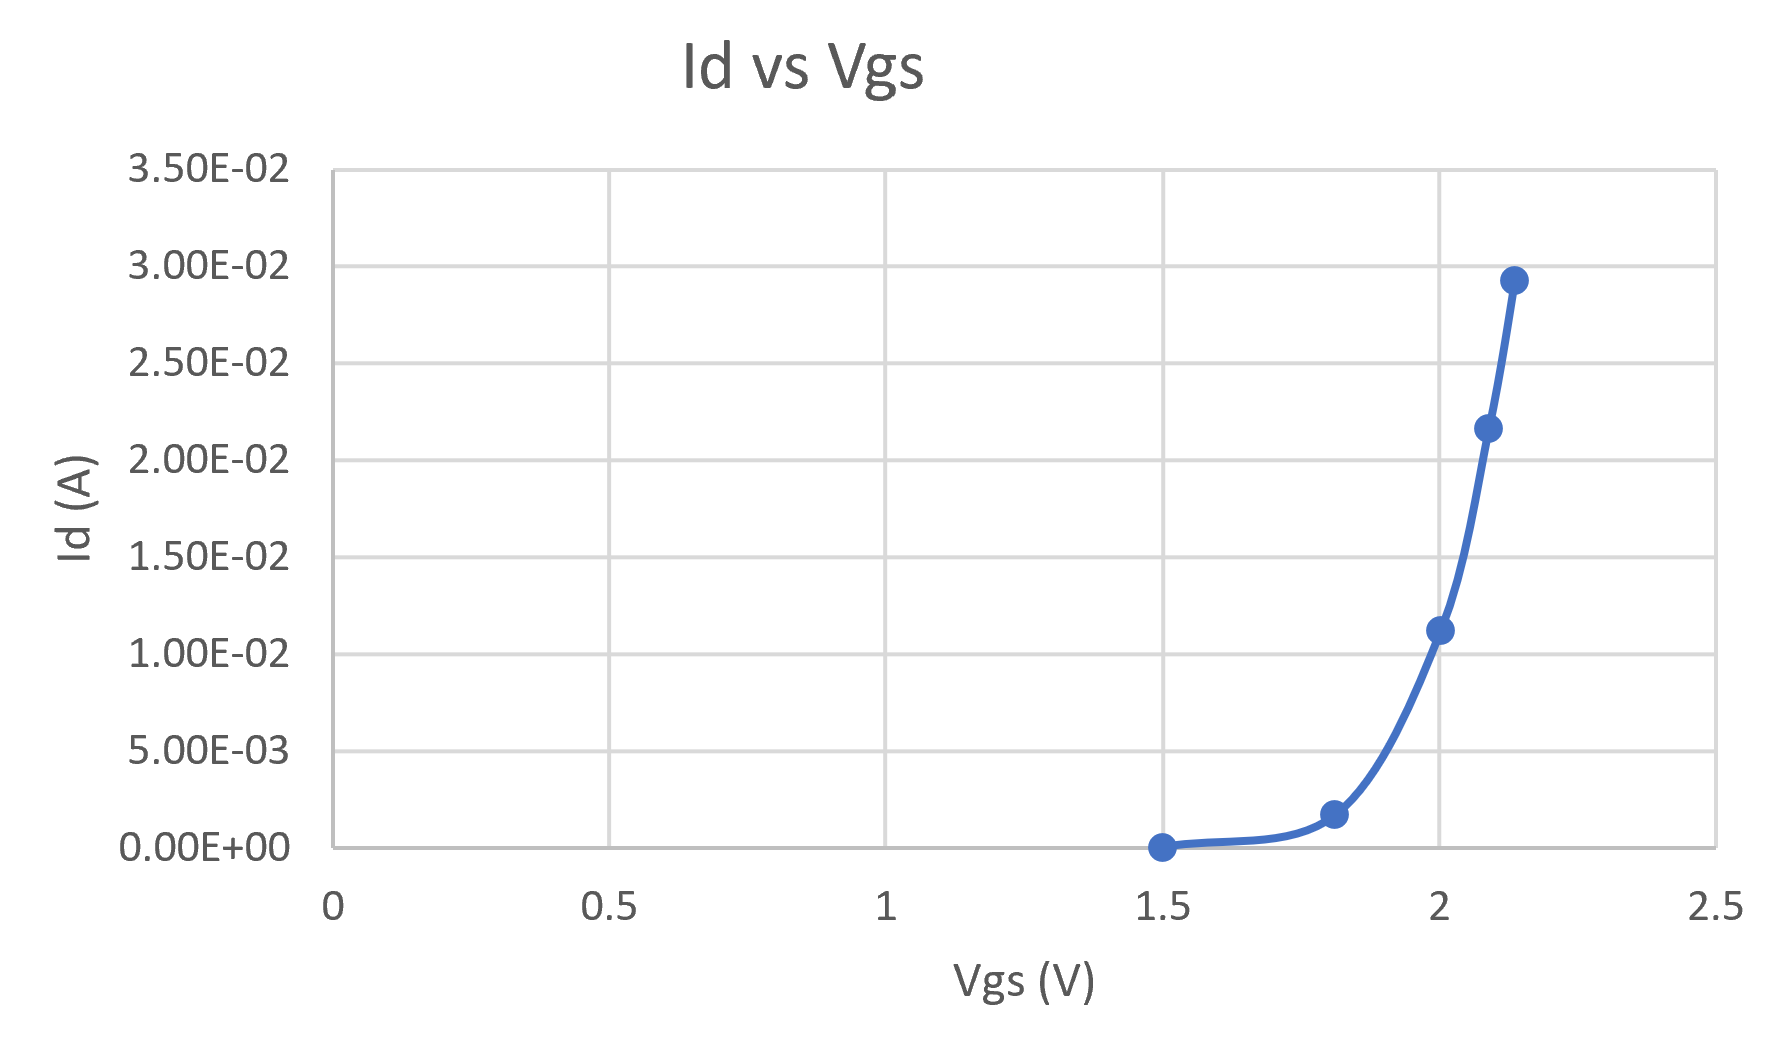
\includegraphics[width=\textwidth]{ECE2200L_Lab7_IV_1.png}
  \caption{$I_D$ vs $V_{GS}$ of circuit 1 at $V_{DS} = \SI{5}{\volt}$}
  \label{fig:IV1}
\end{figure}
\begin{figure}[H]
  \centering
  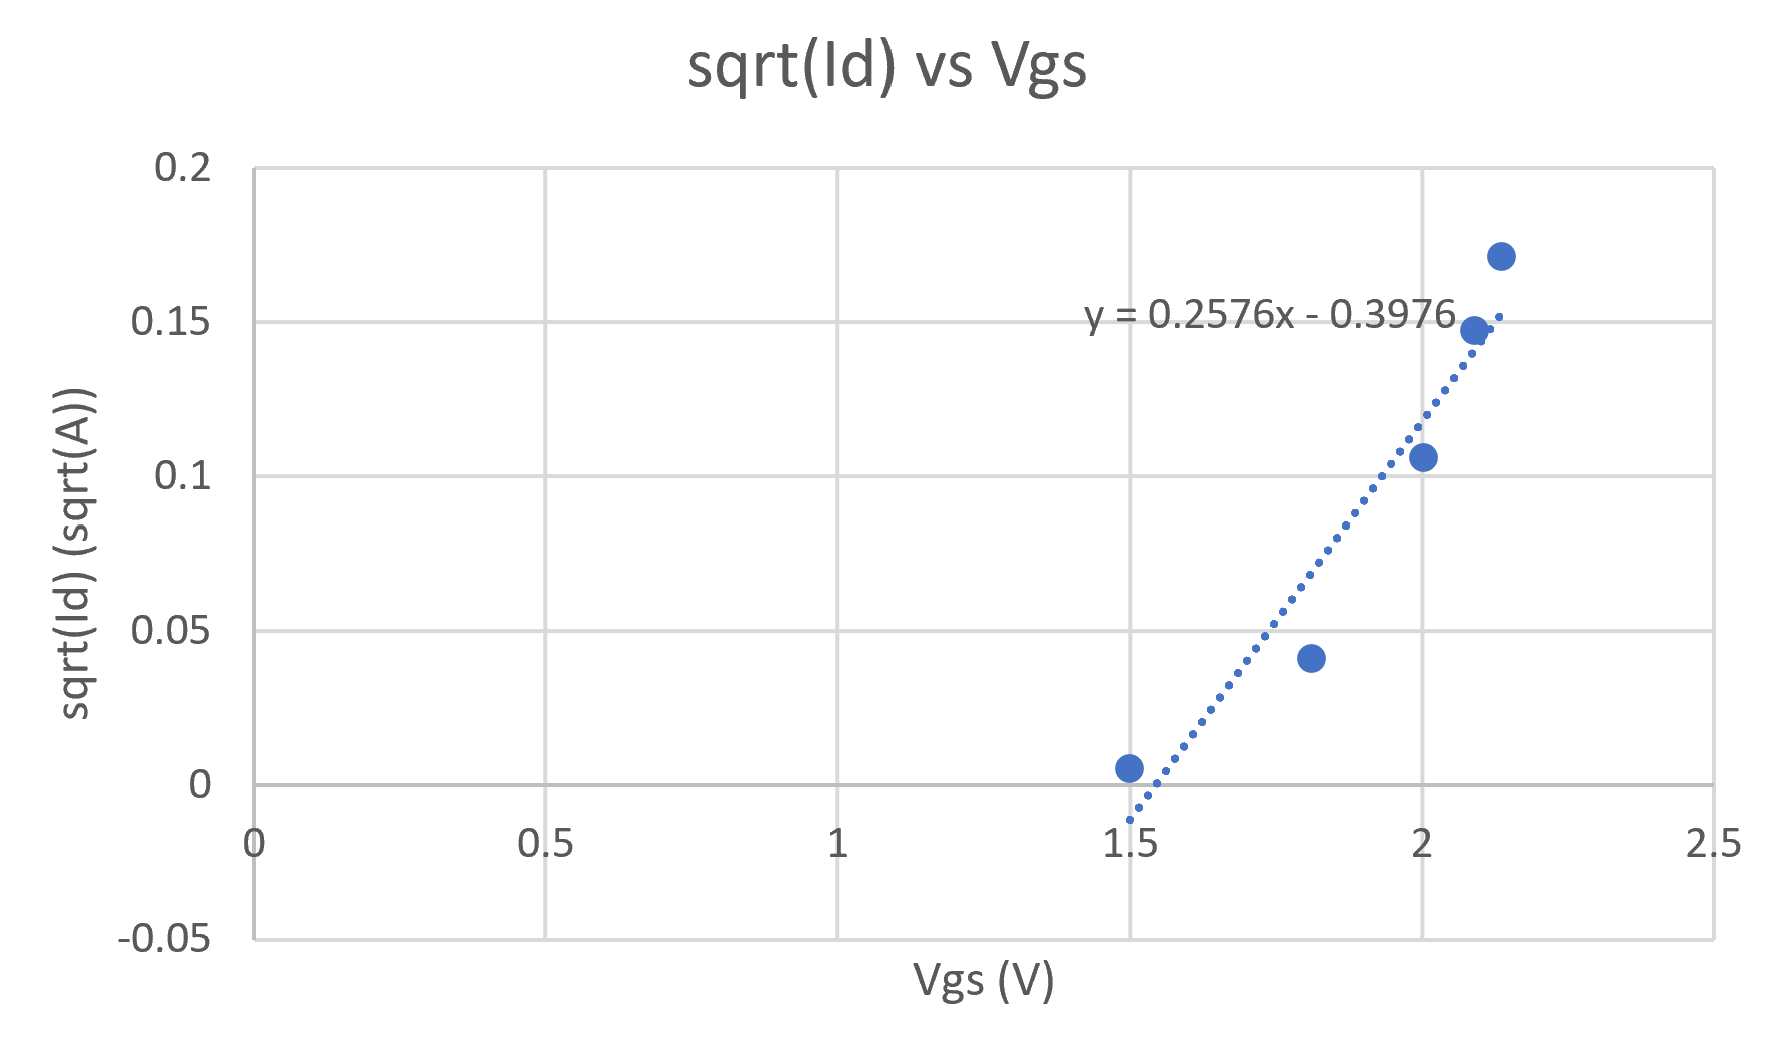
\includegraphics[width=\textwidth]{ECE2200L_Lab7_sqrt.png}
  \caption{$\sqrt{I_D}$ vs $V_{GS}$ of circuit 1 at $V_{DS} = \SI{5}{\volt}$}
  \label{fig:sqrt}
\end{figure}

The above charts demonstrates the MOSFET behavior according to the below equations:
\begin{align}\label{eqn:ckt1}
  I_D&=\frac{K_n}{2}\left(V_{GS}-V_{TH}\right)^2\\
  \sqrt{I_D}&=\sqrt{\frac{K_n}{2}}V_{GS}-\sqrt{\frac{K_n}{2}}V_{TH}
\end{align}
We can then derive $V_{TH}$ from the trendline of figure \ref{fig:sqrt}:
\begin{align}\label{eqn:calc1}
  \sqrt{\frac{K_n}{2}}&=0.2576\;\text{A}^{\frac{1}{2}}\text{V}^{-1}\\
  V_{TH}&= \frac{0.3976}{\sqrt{\frac{K_n}{2}}}=\frac{0.3976}{0.2576}=\SI{1.543}{\volt}
\end{align}

\newpage

\begin{table}[H]
  \caption{$I_D$ vs $V_{DS}$ of circuit 2 at $V_{DS} = \SI{1.817}{\volt}$ and $V_{DS} = \SI{2.001}{\volt}$}
  \begin{minipage}[t]{0.5\textwidth}
    \centering
    $V_{DS} = \SI{1.817}{\volt}$\\
    \vspace{1mm}
    \begin{tabular}{rr}
      \toprule
       $V_{DS}$ (V)&$I_D$ (A)\\
      \midrule
      0.0203 & $4.70\times10^{-4}$ \\
      0.0493 & $9.00\times10^{-4}$ \\
      0.1    & $1.23\times10^{-3}$ \\
      0.2    & $1.40\times10^{-3}$ \\
      0.4    & $1.48\times10^{-3}$ \\
      1      & $1.52\times10^{-3}$ \\
      2      & $1.56\times10^{-3}$ \\
      3      & $1.59\times10^{-3}$ \\
      4      & $1.62\times10^{-3}$ \\
      5      & $1.66\times10^{-3}$ \\
      6      & $1.69\times10^{-3}$ \\
      7      & $1.73\times10^{-3}$ \\
      8      & $1.76\times10^{-3}$ \\
      9      & $1.81\times10^{-3}$ \\
      10     & $1.85\times10^{-3}$ \\
      11     & $1.89\times10^{-3}$ \\
      12     & $1.94\times10^{-3}$ \\
    \bottomrule
    \end{tabular}
    \end{minipage}
    \begin{minipage}[t]{0.5\textwidth}
      \centering
      $V_{DS} = \SI{2.001}{\volt}$\\
      \vspace{1mm}
      \begin{tabular}{rr}
        \toprule
         $V_{DS}$ (V)&$I_D$ (A)\\
        \midrule
        0.024 & $2.07\times10^{-3}$ \\
        0.05  & $3.88\times10^{-3}$ \\
        0.1   & $6.21\times10^{-3}$ \\
        0.2   & $8.29\times10^{-3}$ \\
        0.4   & $9.24\times10^{-3}$ \\
        1     & $9.79\times10^{-3}$ \\
        2     & $1.04\times10^{-2}$ \\
        3     & $1.09\times10^{-2}$ \\
        4     & $1.14\times10^{-2}$ \\
        6     & $1.26\times10^{-2}$ \\
        8.08  & $1.43\times10^{-2}$ \\
        10.04 & $1.62\times10^{-2}$ \\
        11.91 & $1.80\times10^{-2}$ \\
      \bottomrule
    \end{tabular}
    \end{minipage}
  \label{tab:ckt2}%
\end{table}

\begin{figure}[H]
  \centering
  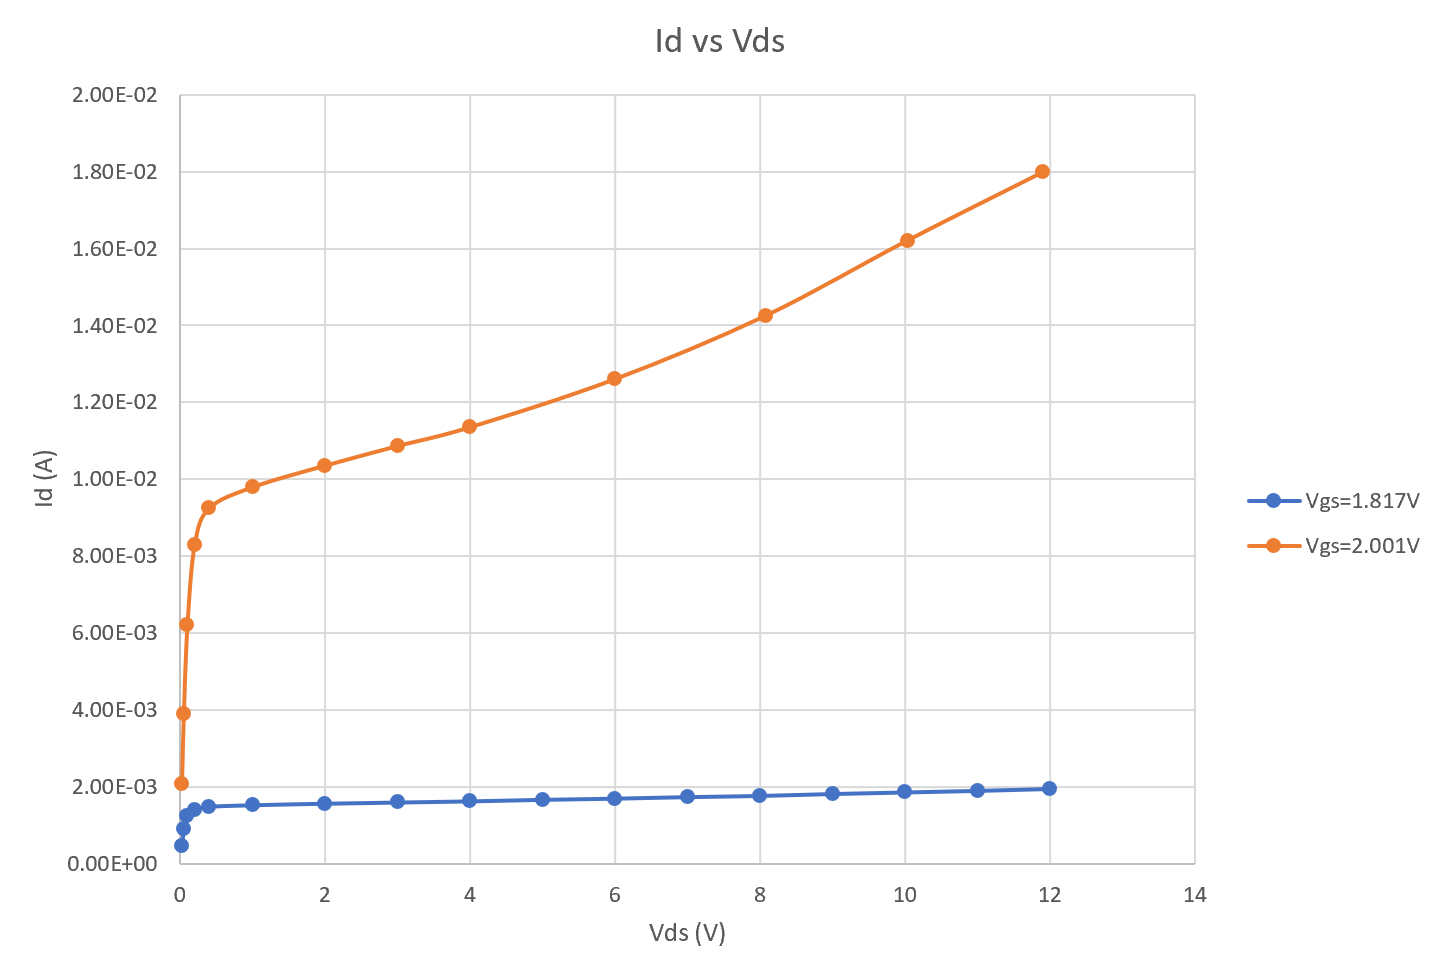
\includegraphics[width=\textwidth]{ECE2200L_Lab7_IV_2.png}
  \caption{$I_D$ vs $V_{DS}$ of circuit 2 at $V_{DS} = \SI{1.817}{\volt}$ and $V_{DS} = \SI{2.001}{\volt}$}
  \label{fig:IV2}
\end{figure}

\begin{figure}[H]
  \centering
  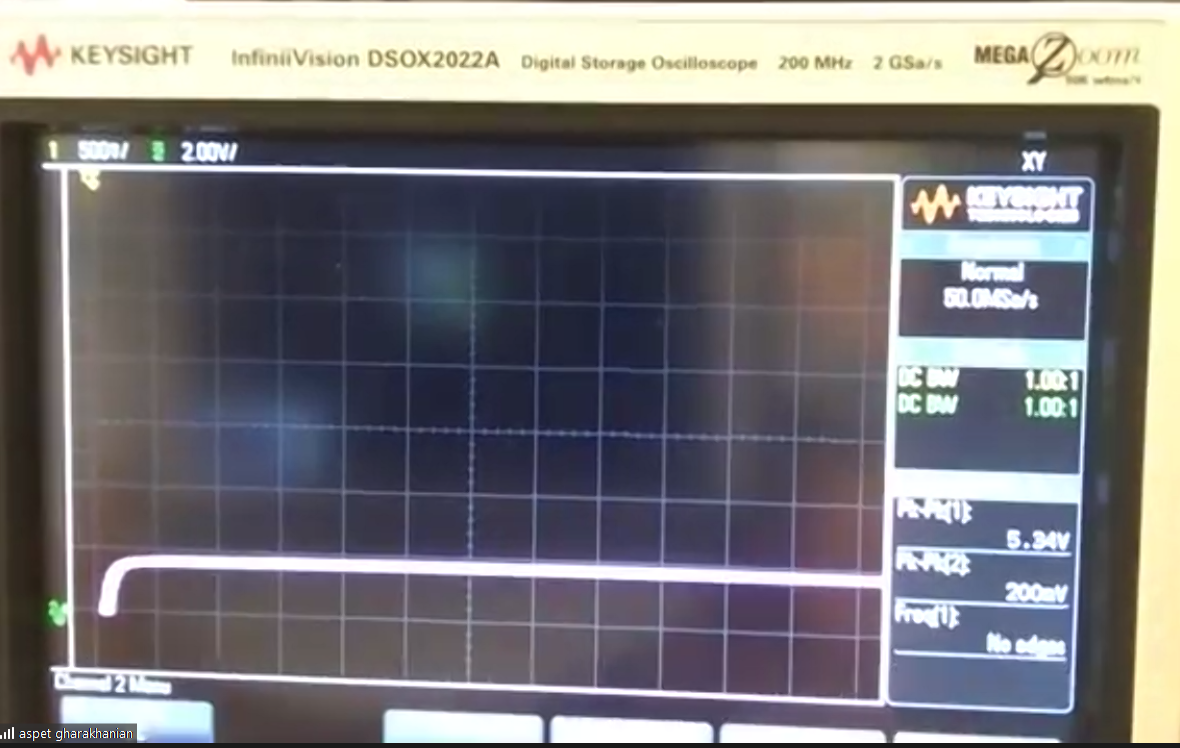
\includegraphics[width=\textwidth]{ECE2200L_Lab7_scope_1.817.png}
  \caption{Oscilloscope display of $I_D$ vs $V_{DS}$ of MOSFET at a lower $V_{DS}$}
  \label{fig:scope1}
\end{figure}

\begin{figure}[H]
  \centering
  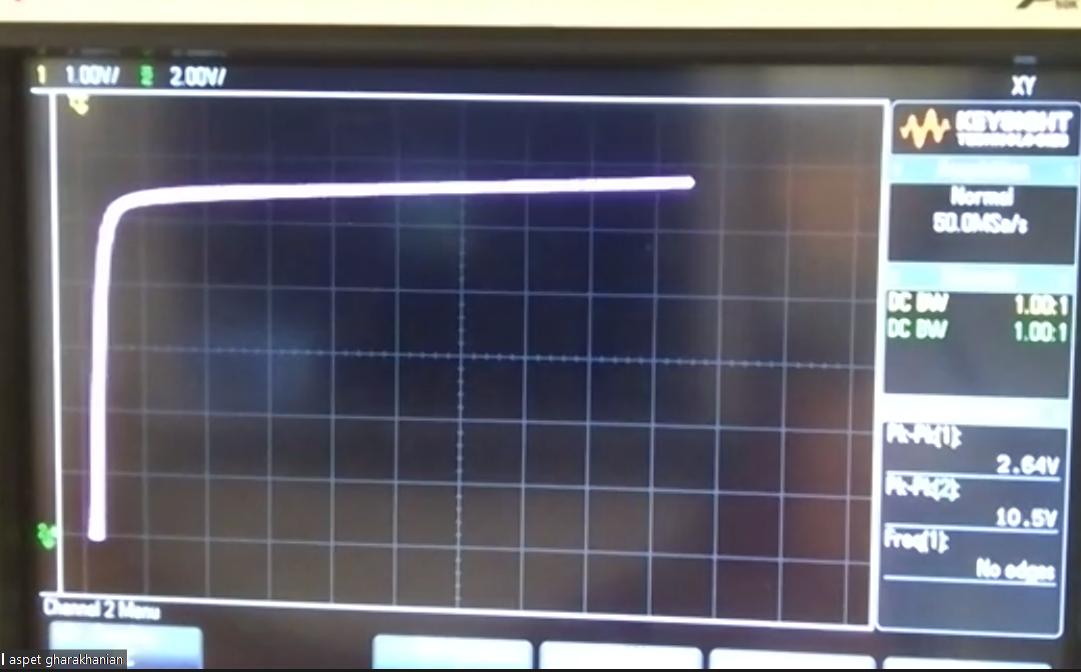
\includegraphics[width=\textwidth]{ECE2200L_Lab7_scope_2.001.png}
  \caption{Oscilloscope display of $I_D$ vs $V_{DS}$ of MOSFET at a higher $V_{DS}$}
  \label{fig:IV2}
\end{figure}


\section*{Conclusion}
As demostrated above, increase of $V_{GS}$ results in an increase in $I_D$ as a function of $V_{DS}$ and the rate of change of $I_D$ with respect to $V_{DS}$.
\end{document}
